\documentclass{article}

%change the margin of the paper
%\usepackage[legalpaper, margin=0.1in]{geometry}
%using the \substack
\usepackage{amsmath}
% \mathbbm{}
\usepackage{bbm}

% NOTE \pdv  partial differential equation
\usepackage{physics}



% hyperlink Here
\usepackage{hyperref}
\hypersetup{
    colorlinks=true,
    linkcolor=blue,
    filecolor=magenta,
    urlcolor=cyan,
}

% this is the package for block comment \begin{comment} and \end{comment}
\usepackage{verbatim}
\usepackage{imakeidx}
% For multiple rows in tabular environment.
\usepackage{multirow}
% use this package to strikeout the word /st{}
%the color package is for the \textcolor{red} to highlight the text
\usepackage{color,soul}
% to define newcolumntype and \arraybackslash
\usepackage{array}
% hyperref is to call /url. hyphen packege to avoid that the url is too long
\PassOptionsToPackage{hyphens}{url}\usepackage{hyperref}
%Todo list, \newlist \setlist...
\usepackage{enumitem,amssymb}
\newlist{todolist}{itemize}{2}
\setlist[todolist]{label=$\square$}

% for image inserting
\usepackage{graphicx}
\graphicspath{./Desktop/Homework/123/7/}
\usepackage{subfig}

% \iff \leqlsant
\usepackage{amssymb}



% Code block begin(lstlisting) and end(lstlisting)
\usepackage{listings}
\usepackage{color}

\definecolor{dkgreen}{rgb}{0,0.6,0}
\definecolor{gray}{rgb}{0.5,0.5,0.5}
\definecolor{mauve}{rgb}{0.58,0,0.82}


%NOTE: Change the "language" parameter here
\lstset{frame=tb,
  language=Matlab,
  aboveskip=3mm,
  belowskip=3mm,
  showstringspaces=false,
  columns=flexible,
  basicstyle={\small\ttfamily},
  numbers=none,
  numberstyle=\tiny\color{gray},
  keywordstyle=\color{blue},
  commentstyle=\color{dkgreen},
  stringstyle=\color{mauve},
  breaklines=true,
  breakatwhitespace=true,
  tabsize=3
}

% Macros
%%%%%%%%%%%% Text Color %%%%%%%%%%%%%%%
\definecolor{mypink1}{RGB}{219, 48, 233}
\definecolor{myred1}{RGB}{231, 76, 60}
\definecolor{myred2}{RGB}{203, 67, 53}
\definecolor{myblue1}{RGB}{52, 152, 219}
\definecolor{mygray}{gray}{0.6}

%% Table Style
\newcolumntype{C}{>{\center\arraybackslash}m{.70\columnwidth}}
\newcolumntype{Y}{>{\center\arraybackslash}m{2cm}}



%NOTE title Here
\title{Homework 7}
\author{Hanyuan Zhu}


\begin{document}
\subsection*{ Question 1}

\paragraph{a.}
$c_{r}^{i} = [-\frac{r}{2}, \frac{r}{2}]$ is the interval of ith dimension of cube $C_{r}^{D}$.

Because $ Vol_{D} A = \int_{A} dx_1 ... dx_D $,

\begin{equation}
  \begin{split}
    Vol_{D} (C_{r}^{D}) &= \int_{C_{r}^{D}} dx_1 ... dx_D\\
    &= \int_{c_{r}^{D}} ...\int_{c_{r}^{1}} dx_1 ... dx_D\\
    &= \prod_{i = 1}^{D} \int_{c_{r}^{i}} dx_i\\
    &= \prod_{i = 1}^{D} r = r^D
  \end{split}
\end{equation}

\paragraph{b.}

Since $ A_{\epsilon, r}^{D} = \{ xC_{r}^{D}| x \not\in C_{\epsilon}^{D} \} = C_{r}^{D} - C_{r - \epsilon}^{D} $,
\begin{equation}
  \begin{split}
    Vol_{D} (A_{\epsilon, r}^{D}) &= \int_{A_{\epsilon, r}^{D}} dx_1 ... dx_D \\
    &= \int_{C_{r}^{D} - C_{r - \epsilon}^{D}} dx_1 ... dx_D\\
    &= \int_{C_{r}^{D} } dx_1 ... dx_D - \int_{ C_{r - \epsilon}^{D}} dx_1 ... dx_D\\
    &= r^D - (r-\epsilon)^D
  \end{split}
\end{equation}

Then $ \frac{Vol_{D} (A_{\epsilon, r}^{D})}{Vol_{D} (C_{r}^{D})} = \frac{r^D - (r-\epsilon)^D}{r^D} = 1 - (1- \frac{\epsilon}{r})^D$

\paragraph{c.}

When $D = 10$, if $ \epsilon = \frac{r}{10}$, $\frac{Vol_{D} (A_{\epsilon, r}^{D})}{Vol_{D} (C_{r}^{D})} = 65.13 \% $.

Because $ 0 < \epsilon < r $, $1 -\frac{\epsilon}{r} <1 \text{ and } \frac{r}{r-\epsilon}>1$
\begin{equation}
  \begin{split}
    \pdv{}{D} (\frac{Vol_{D} (A_{\epsilon, r}^{D})}{Vol_{D} (C_{r}^{D})}) &= - \pdv{}{D} (1- \frac{\epsilon}{r})^D\\
    &= ln(\frac{r}{r-\epsilon})(1- \frac{\epsilon}{r}) >0
  \end{split}
\end{equation}
It means that the ratio $\frac{Vol_{D} (A_{\epsilon, r}^{D})}{Vol_{D} (C_{r}^{D})}$ monotonically increases as D get larger.

\subsection*{ Question 2}

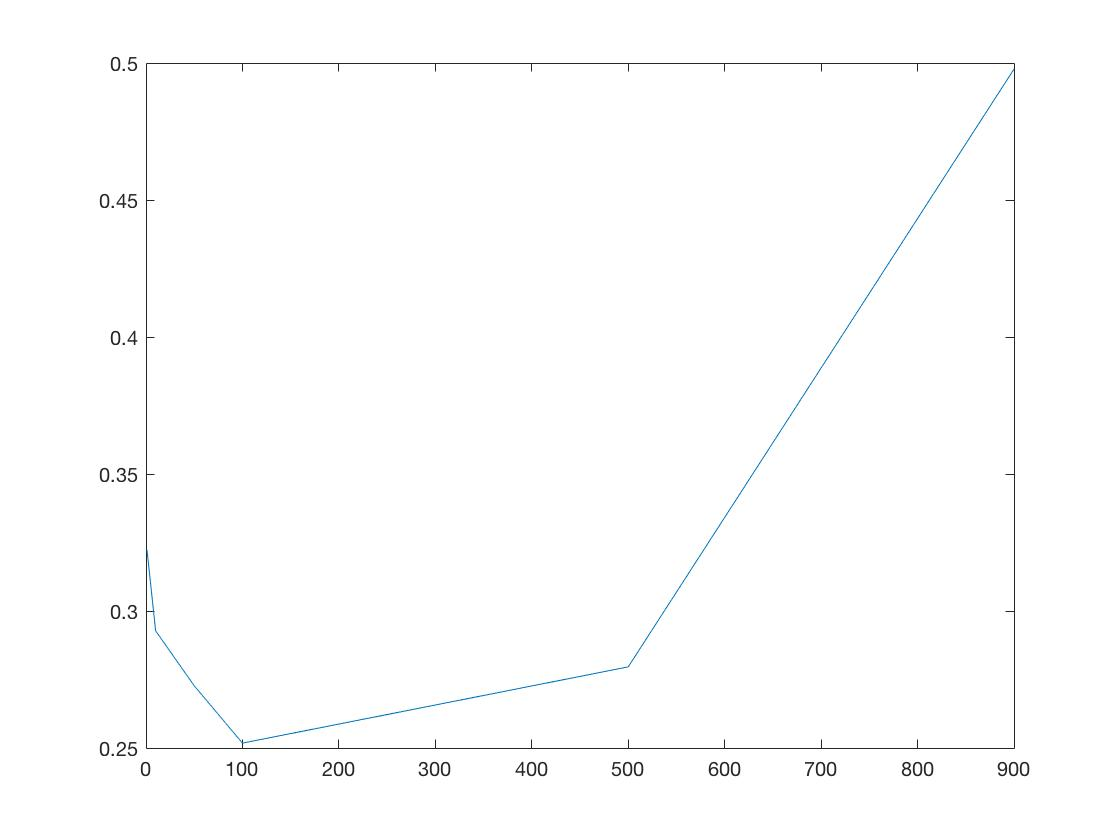
\includegraphics[width=8cm, height=8cm]{Code/q2}

The kNN of best performance among this kNN set,$ \{ 1, 10, 50, 100, 500, 900\} $ , is at kNN $= 100$.
When kNN is too small, the model will be underfitting; when kNN is too large, the model will be overfitting.

The code will be attached at the end.




\subsection*{ Question 3}

\begin{figure}[h]
  \centering
  \subfloat[ Epoch 1 ]{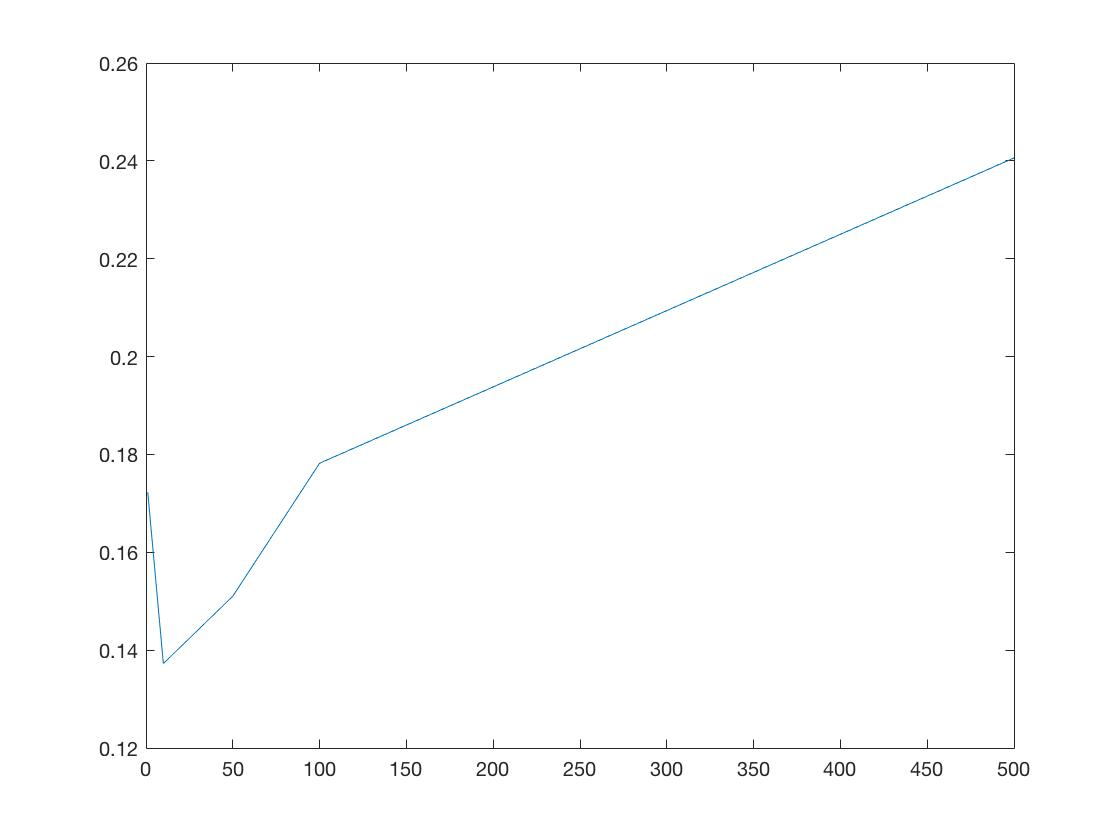
\includegraphics[width=4cm, height=4cm]{Code/q3}}
  \qquad
  \subfloat[ Epoch 2 ]{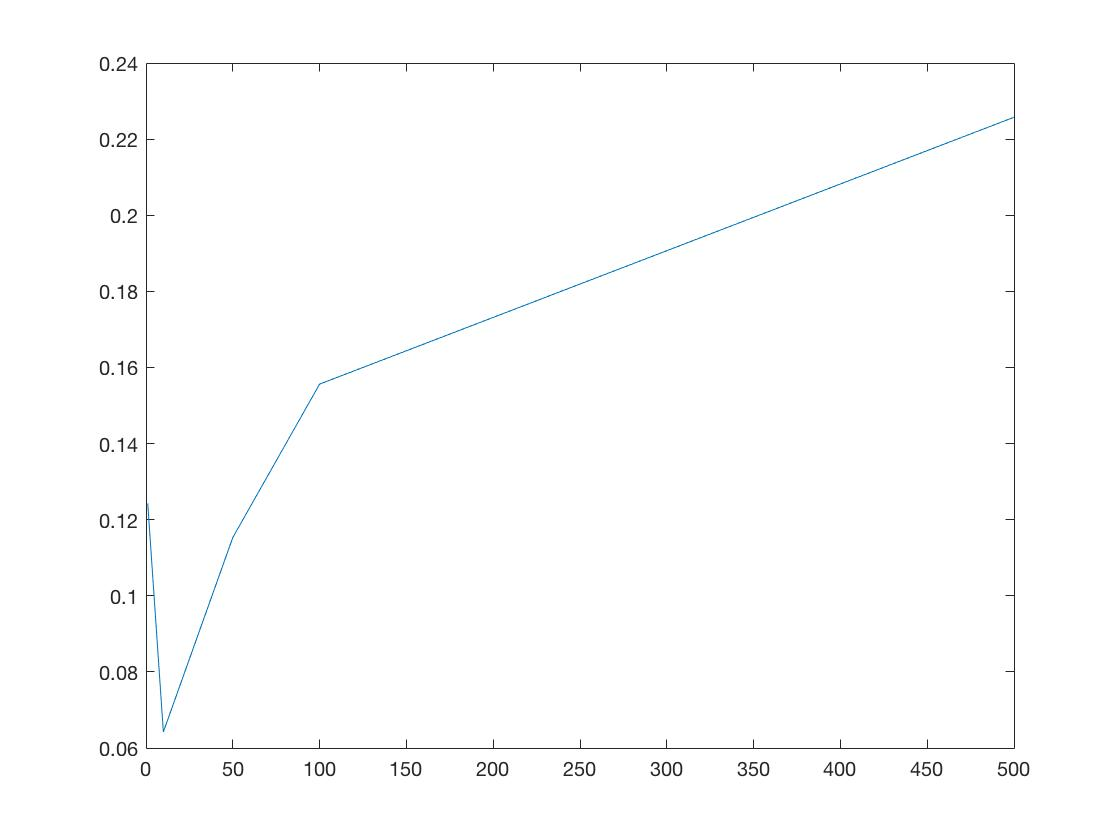
\includegraphics[width=4cm, height=4cm]{Code/q32}}
  \qquad
  \subfloat[ Epoch 3 ]{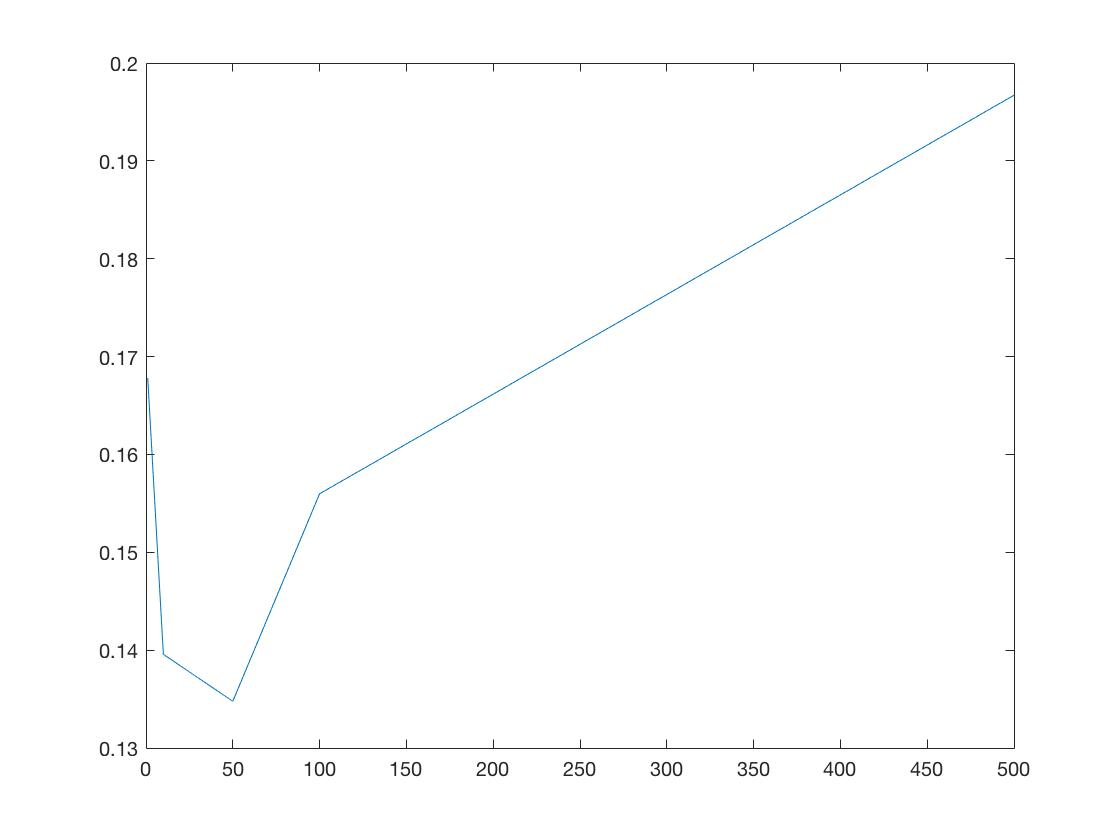
\includegraphics[width=4cm, height=4cm]{Code/q33}}
  \qquad
  \subfloat[ Epoch 4 ]{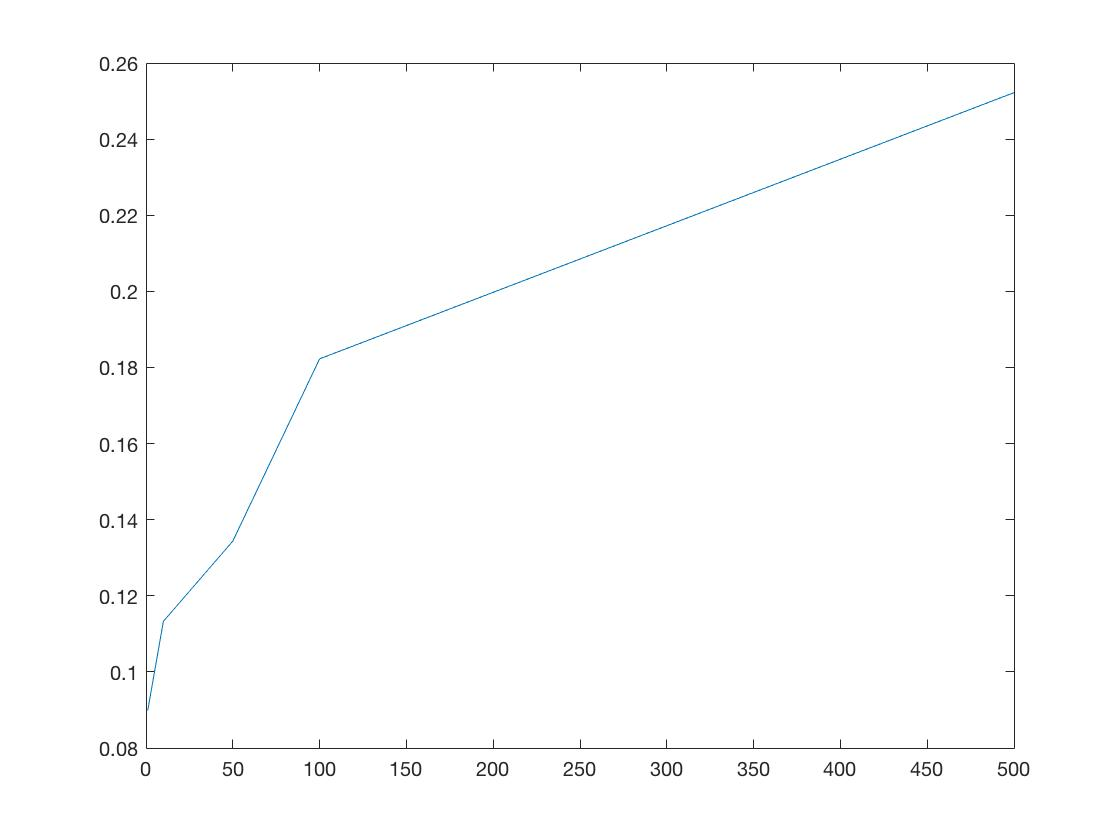
\includegraphics[width=4cm, height=4cm]{Code/q34}}
\end{figure}

Basing on the results from 10 epoches ( below only shows 4 of 10 epoches), when the kNN is smaller 100,
the loss will be small. Sometimes when kNN is 1, loss will be relatively large, because a large amount testing points is at boundary of the partitions.

The code will be attached at the end.

\newpage


\subsection*{ Question 4}
\paragraph{a.}
$  E = \{ x \in \mathbbm{R}^d | w^T x = 0\} $, it means E is nullspace of $w^T$, $E=Null(w^T)$

Because $w^T \in \mathbbm{R}^d$ and $ w^T \neq 0$
\begin{equation}
  dim(E) = dim( \mathbbm{R}^d ) - dim(w^T) = d - 1
\end{equation}

\paragraph{b.}
Part (a) has proved that $S = \{ x \in \mathbbm{R} | w^T x = 0\} $ has rank $d-1$.
We can rewrite S as below

\begin{equation}
  \begin{split}
    S &= \{ (x+v)\in \mathbbm{R}^d | w^T (x + v) = 0 , \text{for some } v \in \mathbbm{R}^d \text{ s.t. }  w^T v = - b    \}\\
    &= \{ (x+v)\in \mathbbm{R}^d | w^T x = b , \text{for some } v \in \mathbbm{R}^d \text{ s.t. }  w^T v = - b    \}
\end{split}
\end{equation}

Now $E = \{ x \in \mathbbm{R}^d | w^T x = b\}$ is isomorphic to S by \textbf{a translation}, that is
$$ E = \{x \in \mathbbm{R}^d | x = y - v \text{ for } y \in S \text{ and some } v \in \mathbbm{R}^d \text{ s.t. }  w^T v = - b  \}$$

Thus E has same dimension as S, that is $ d - 1$.

\subsection{Code of Question 2}
\begin{lstlisting}
  load kNN_ClassifierSyntheticData
% Labels: 1x1000 lebels
% X : 1000X2 Data point


%% Random sample data

XLabels = [X Labels.'];

testidx = randperm(1000,100);

test100 = XLabels(testidx,:) ;

trainidx = setdiff([1:1000],testidx);

%training set
train900 = XLabels(trainidx,:) ;

samX= train900(:,1:2);
samL= train900(:,3);

%initiate data
kNNset = [1 10 50 100 500 900];
Loss100 =[];

%% Model builder

for kNN = kNNset
    Mdl = fitcknn(samX,samL,'NumNeighbors',kNN);
    Loss100 = [Loss100 loss(Mdl,test100(:,1:2),test100(:,3))];
end
\end{lstlisting}

\begin{lstlisting}
load SalinasA_gt
load SalinasA


%% Random sample data

lineSal = reshape(salinasA,[],224);
lineGT = reshape(salinasA_gt,[],1);

XLabels = [lineSal lineGT];

%test set
testidx = randperm(length(XLabels),100);

test100 = XLabels(testidx,:) ;

%training set
trainidx = setdiff([1:length(XLabels)],testidx);

trainSet = XLabels(trainidx,:) ;

samX= trainSet(:,1:224);
samL= trainSet(:,225);

%initiate data
kNNset = [1 10 50 100 500];
Loss100 =[];

%% Model builder

for kNN = kNNset
    Mdl = fitcknn(samX,samL,'NumNeighbors',kNN);
    Loss100 = [Loss100 loss(Mdl,test100(:,1:224),test100(:,225))];
end
\end{lstlisting}


\end{document}
